\documentclass[12pt]{article}
\usepackage{times}
\usepackage{rotating}
\usepackage{setspace}
\doublespacing
\usepackage[letterpaper]{geometry}
\geometry{top=1.0in, bottom=1.0in, left=1.0in, right=1.0in}
\usepackage{dirtytalk}
\usepackage{csquotes}
\setlength\headsep{0.333in}
\usepackage{graphicx}
\usepackage{subcaption}
\usepackage{fancyhdr}
\pagestyle{fancy}
\lhead{}
\chead{}
\rhead{Gupta \thepage}
\lfoot{}
\cfoot{}
\rfoot{}
\renewcommand{\headrulewidth}{0pt}
\renewcommand{\footrulewidth}{0pt}

\newcommand{\bibent}{\noindent \hangindent 40pt}
\newenvironment{workscited}{\newpage \begin{center} Works Cited \end{center}}{\newpage }

\newenvironment{coverletter}{\begin{center} Cover Letter \end{center}}{\newpage }
\DeclareTextFontCommand{\booktitle}{\em}


\begin{document}
\begin{flushleft}


\begin{spacing}{2.0}
Harshita Gupta

Humanities Colloqium

April 26, 2017

\begin{coverletter}
\singlespacing

My conversation with Professor Miller helped to identify some key concerns with the experiments I was engaging in and why this was causing difficulty in interpretation. As he put it, I had ``too many degrees'' to my experiments, and was applying the meta-processes of close reading to experimental, almost scientific exploration, which needed, as he said, ''more controls``. I reduced the translations I was dealing with, reduced the role of the graphs and visuals in my interpretation, and focused on using preexisting analyses as my axes upon which to make interpretive moves or pivots. 

In developing this revision, I used Franco Moretti's ``Network Theory, Plot Analysis'' from \booktitle{Distant Reading} as a model of a work in a similar genre. The day after our conference, I was finally able to get my network code to work, and figured out how to visualize topics as a graph connecting different words and elements across texts. This gave me a very productive experimental setup for understanding what I'd been interested in all along, the unique thematic 'structure' of each of the texts. As Moretti says in his analysis of Hamlet through a network of its plot,

\begin{displayquote}
Finally - and it is the most important thing of all, but also the most difficult - one can intervene on a model; make experiments. Take the protagonist again. For literary critics, this figure is important because it is a very meaningful part of the text; there is always a lot to be said about it; we would never think of discussing Hamlet—without Hamlet. But this is exactly what network theory tempts us to do: take the Hamlet-network, and remove Hamlet, to see what happens.
\end{displayquote}

I engage in this process of "making experiments" on the networks that I produce, by deleting different variations of words like 'women', 'daughter', 'mother', and 'mistress', and subsequently understanding their effect on the network: to put it differently: I attempt to understand each translation with questions like ``What remains of the of each translation's depiction of women when we remove mentions of all male - associated women, like mothers, wives, and daughters?'' ``Do women remain in the networks, and to what extent, when we remove mentions of courtly duties and performance, versus when we remove mentions of feeling, emotion, and thought?'' How does each translation's network respond differently to these interventions? Engaging with the models in this way was the most challenging part of HUM10 all year, since it was unlike anything I've done before; it was very difficult to think of productive questions that would reveal interesting trends, write code to answer the questions, wait for it to run, and analyze my results thoughtfully without getting lost in the 80 or so files that each run of code would generate. \linebreak

When I cleaned the models according to the interests I expressed in draft, removing some rogue proper nouns and publishers notes, many of the trends that I'd identified in my draft, like the difference in occurrences of women, were no longer present. Generating the models with the parts of speech that I detected earlier, and with the topic number setting set to 15, also yielded cleaner, more meaningful topics that didn't have as many unreadable words or errors. Additionally, instead of simply using the top ten words in a topic, I used a threshold value to determine whether the topics coherence was statistically significant (threshold signal value); I felt like this was a representation that relied on a more rigorous understanding of the model's output.\linebreak

I think much of the difficulty with this paper was that I'm not as well trained in reading and interpreting models as I am in close-reading --- setting out on this project was a challenge in both, the model-creation respect, as well as in learning to productively and accurately interpret topic signals and force-directed network graphs. \linebreak

Given more time and resources, I would certainly give these models and their results a more thorough treatment, with perhaps a more ``mesoanalytic'' lens --- since I wasn't able to read all four translations in depth, and was only interacting with models, the traditionalist in me (however small a part that may be) finds the result only partly satisfying. I would want to endeavor to correlate my network's results with clearer plot and thematic trends across the text, versus ones in specific scenes that the topics can point out; this would only be doable once I've read the entirety of each text.

\end{coverletter}


\begin{center}
Title
\end{center}

\setlength{\parindent}{0.5in}

In Metonymy in The Tale of Genji: An Analysis of Translation Strategies, Janel R. Goodman Murakami compares occurrences of metonymy in a passage across translations of the Tale of Genji to assess how domesticated or foreignized Suematsu's, Waley's, Seidensticker's, and Tyler's translations are, concluding that the more modern translators retain foreign elements of the text more faithfully than their earlier counterparts. In ``Going to Bed with Waley: How Murasaki Shikibu does and does not become world literature,'' Valerie Henitiuk uses a similar microanalytic approach, more commonly referred to as close-reading, to analyze the scene of Genji's and Murasaki's consummation. She argues that while Seidensticker's  portrayal of the scene as rape and an act of aggression may initially appear feminist and progressive, portraying the scene as such an out-of-sorts one, it loses the opportunity to employ the ``far more subtle and thus profound criticism... to explore the insidious social problems at the very root of situations like this'' (Henitiuk 56). Seidensticker's portrayal, as well as Tyler's (though to a lesser extent), emphasizes the difficulties of the specific situation over the system at large, missing the larger social commentary that Murasaki Shikibu is making, or the ``true critique being leveled at prevailing attitudes and behaviors''. A successful critique, would be ``implicit but no less scathing'' (Henitiuk 57).

Henitiuk's conclusions are drawn based on close readings of a select few passages from each translation, a very microscopic approach for a text as varied and large in scope as \booktitle{Genji}. Her argument is based on the understanding that Seidensticker and Tyler misstep by setting apart this scene from the rest of the novel; Henitiuk is thereby relying on a fundamentally macroanalytic understanding of each translation's baseline for representing interactions amongst characters. This is where a definitively macroanalytic approach offered by computational analysis is useful. My paper draws out and tests the underlying assumptions to Henitiuk's microanalysis by offering a holistic, modeled understanding of each translation's thematic world to shed light on the portrayal of the morning-after scene in juxtaposition to the text as a whole. I ultimately discover TODO

In my endeavor to, like Murakami, evaluate the thematic and linguistic domestication versus foreignization of a translation, I turn to a work referenced by Henitiuk in ``Going to Bed With Waley,'' Margaret H Childs' ``The Value of Vulnerability: Sexual Coercion and the Nature of Love in Japanese Court.'' Childs analyzes the ``cross-cultural emotional experience'' and highlights the difference between modern American expectations of love and premodern Japanese literary representations of it. Her preliminary statements are about general categories of emotion, drawing attention to studies that show that the American schemas of emotion differ from Chinese ones in their inclusion of surprise, while Chinese ones differ from the American in their inclusion of shame, but the crux of her discussion is around the un-American category of loving feelings called 'sad love' depicted in Japanese literature, which is associated with negative emotions and words like 'pity' and 'pathetic'. There is a high correlation between fragility and beauty, and vulnerability and attraction.

Using Childs' research to set up these measurable variables to determine the ``westernization'' of a text --- through its cooccurring depiction of love and negative emotion --- sets the stage for technical models to take over and offer information about where each text falls on the spectrum of domestic to foreign. The appropriate tool for an analysis of negative emotion is sentiment analysis, a natural language processing tool that determines the positive or negative polarity of a word. I conducted sentiment analyses on the three translations in concern and displayed a histogram of the results for each text. \footnote{All sentiment scores with an absolute value of less than 0.0001 were excluded from the graphs, since they provide no interpretive value.}

\begin{figure}
	\begin{subfigure}{.3\linewidth}
		\includegraphics[width=2in]{seidensticker-sentiment.png}\hfill
		\caption{\scriptsize Median: 0.23, Mean: 0.04, Variance: 0.1772}
	\end{subfigure}
	\begin{subfigure}{.3\linewidth}
		\includegraphics[width=2in]{tyler-sentiment.png}\hfill
		\caption{\scriptsize Median: 0.28, Mean: 0.06, Variance: 0.067}		
	\end{subfigure}
	\begin{subfigure}{.3\linewidth}
		\includegraphics[width=2in]{washburn-sentiment.png}
		\caption{\scriptsize Median: 0.28, Mean: 0.04, Variance: 0.0772}
	\end{subfigure}
    \caption{Positive and Negative Sentiment Across \booktitle{Genji}}
    \label{sentiment-hists}
\end{figure}

An analysis of the histograms, along with the mean, median, and variance of the data, shows that Seidensticker's text is markedly more variant in its depiction of emotion, with a heavier clustering of values towards the edges of the graph than the other two texts. All the graphs have a much smaller mean than a median, which shows that the mean is skewed by some very low sentiment scores --- this is no surprise, as any reader of \booktitle{Genji} can surmise that the book is rife with dramatic, often heart-wrenching emotion. The presence of negative emotion in a plot filled with romantic entanglements suggests that the texts are reasonably close to Childs' understanding of Eastern-language texts' depictions of love, but a simple sentiment analysis reveals only the presence of negative emotion across the entirety of the text's plot, not that it occurs in romantic contexts. To determine whether there is meaningful cooccurrence between negative-sentiment-scoring words and love, or in other words, whether the translation is true to ``sad love,'' I turn to topic modeling. 

I apply digital topic modeling to break down and analyze the three translations of Genji in concern: Edward G. Seidensticker's from 1976, Royall Tyler's from 2001, and Dennis Washburn's from 2015 \footnote{ My greatest interest was originally in comparing the work of male translators with Helen McCullough's partial translation. Unfortunately, McCullough's translation, published only in \booktitle{Genji and Heike: selections from the Tale of Genji and the Tale of the Heike}, is heavily copyrighted and unavailable in any digital format.}. Topic modeling is a natural language processing technique that uses the principle of distributional semantics, or the common cooccurrence of two words, to group words into ``topics.'' I use the Latent Dirichlet Allocation (LDA) topic modeling method, which operates on 1000-word sequential chunks of the tale of Genji. LDA treats each ``chunk'' of words as an entity composed of ``topics'' --- each topic is composed of words that commonly occur together. A statistical explanation of LDA modeling's assumptions and mechanisms is beyond the scope of this paper, and one can turn to Rhody's ``Unpacking the Assumptions of LDA'' or Jockers' Macroanalysis for a simplified analysis of the method. Crucial to this paper and its discussion, however, is LDA modeling's unsupervised nature. Topics are not produced based on the program's understanding of the words' meanings or potential similarity, but creates buckets for topics based on the position of words relative to each other, and their common cooccurrence, i.e. distributional similarity, to determine that they belong to a similar topic. Its unsupervised nature makes LDA modeling useful for identifying topics in a more ``objective'' fashion by identifying authors' subconscious placement of words and themes and therefore reflecting their gendered and cultural inclinations. Topic modeling is useful, therefore, not just due to ability to give us a zoomed-out, abstracted view of a text as large as Genji, but also in uncovering topics that might be outside our microanalysis-based understanding of discoverable topics.

Topic modeling is traditionally applied to multiple documents that are dissimilar, as in the work by Jockers, and has been trained on corpuses containing multiple texts, 4500 poems in Rhody's case and 4500 texts in Jockers' case. These models develop generalized, often easily identifiable themes that can apply to texts across time and author, like Rhody's ``night light moon stars day dark'' and ``tree green summer flowers grass'' topics. Jockers' and Rhody's topics reveal nothing surprising in their content themselves; the combinations of words are predictable. Topic modeling of the form they practice is useful when the purpose of the topics, albeit predictable, is to be used later in topic distribution comparison across texts, but is less useful when working with a single text. I train the LDA model, instead, on a single translation of Genji at a time, thereby developing topics that are far more specific to each translation's ``thematic world,'' and useful in identifying the thematic differences underlying each translation. The interpretive advantage to this method is evident in the difference between the topics generated by the two cited authors, and the ones I display and analyze in my paper.

\begin{figure}
\caption{Topics in Seidensticker's Translation}
\label{seidensticker-topics}
\singlespacing
\small
Topic 1: stag softer curt outstandingli inwardli recast

Topic 2: seem come said t even see littl bishop dream came child look old girl 

Topic 3: seem robe paint red princess ladi women line littl white string master nose now 

Topic 4: girl ladi said seem thought think come now t look littl even know daughter good young time see women mother make came much go well man way princ 

Topic 5: seem thought even think come see now said go ladi princess time thing littl women make know world long want much day way say made feel look came still noth father 

Topic 6: emperor princ thought seem ladi court chines crown daughter present palac time son said year royal 

Topic 7: princ ladi emperor said blossom kobai daughter thought carriag even 

Topic 8: seem thought women littl governor even young room ladi look light said came back open away door wind way see day veranda 

Topic 9: emperor time now matter tear princ minist empress 

Topic 10: seem ladi safflow quarter white look 

Topic 11: ladi seem thought now time day even said year come see old princess came made much littl 

Topic 12: seem ladi thought daughter year come old think said son day thing well great made man 

Topic 13: t man thing good governor say seem girl think make look know go happen said woman daughter wife one want young day come even just don ve sort someon see everyth peopl m let ask 

Topic 14: emperor ladi court cat princ son crown mother third new father go see royal 
\end{figure}

\begin{figure}
\caption{Topics in Tyler's Translation}
\label{tyler-topics}
\singlespacing
\small
Topic 1: high paper great shoot book write cup scroll command son 

Topic 2: now high even look said way well still thought never time see littl go come long know feel seem day just thing ladi 

Topic 3: play captain old tale now flute music never ladi feel said seem life day hear say even 

Topic 4: majesti now flower light even wind long morn said dew day 

Topic 5: blossom look command made flower ladi littl spring beauti year 

Topic 6: now monk day world holi long mountain come adept wind littl captain thought citi know rever sent look way time 

Topic 7: rever nun young woman lordship go die come mother said even someon tell now noth high see look seem ask never sure just back told heard well happen talk sister women mistress 

Topic 8: majesti flower spring autumn ladi nun music year pine east quarter made consort wing long blossom high garden color 

Topic 9: captain young excel high play look lieuten son music blossom said right just seem man dress one even well make daughter come ladi secretari advis 

Topic 10: even now old play novic high noth often see biwa 

Topic 11: ladi gown look dress comb box one never mistress even high far day now cathay plum 

Topic 12: now long majesti littl thought day mani ladi made year see said well citi time still even come go look 
\end{figure}


\begin{figure}
\caption{Topics in Washburn's Translation}
\label{washburn-topics}
\singlespacing
\small
Topic 1: go ladi just woman feel come girl know even way said make think now nurs tell ask littl man lord night well look time dont attend see thought place 

Topic 2: carriag go feel wife process men view attend ladi just way blind space 

Topic 3: feel husband now even ladi emot heart deep woman say 

Topic 4: made lotu attend third minist flower make 

Topic 5: even capit boat day governor sea attend provinc ladi wind perform lord dream wave 

Topic 6: robe look ladi poem even day garden now seem blossom color tree made women 

Topic 7: cat third princess princ son crown littl blind robe felt see look close game face never contest think tri remark 

Topic 8: even feel now time world look thought see come ladi live heart felt just princess long villa day go 

Topic 9: father hardli wife 

Topic 10: time daughter son even emperor palac princ princess now father court look day year majesti third minist mani feel ladi world left 

Topic 11: play koto string instrument perform princess even music young son boy littl seem flute hear time daughter look major just robe women feel 

Topic 12: woman make way even man young just time now thing matter go mani 

Topic 13: princess even look feel young daughter woman man just ladi now go think women make time way captain letter thought see thing say come still 

Topic 14: ladi wind princess day ceremoni daughter father come carriag 
\end{figure}

Developing meaningful topics is not just a matter of corpus scale, but also of corpus content: following Jockers' guidance, I remove all stop words that do not provide interpretive value, like articles and pronouns, from the corpus before I discover themes within it. In ``Theme'', Jockers proposes and demonstrates topic modeling only on a corpus of common nouns. Restricting the corpus to nouns is appropriate in his use case as his corpus is much larger than a single \booktitle{Genji} translation, and therefore filtering for nouns allows for a higher level of abstraction that focuses on broader trends that are more likely to occur across hundreds of texts. In analyzing \booktitle{Genji}, however, restricting my models to only nouns results in a loss of rich nuance which is central to a cross-translation comparison: adjectives, adverbs, and verbs contain a wealth of information about emotion, description, and subjectivity. To this end, I include adverbs, adjectives, and verbs in my topic models.\footnote{ In addition to removing stop words and parts of speech other than the ones specified, I removed all annotations, introductions, publishers' notes, footnotes, and endnotes. In the Tyler translation, this included the deletion of all chapter titles that are not from the original, chapter introductions, and the ``Persons'' and ``Relationship to Previous Chapters'' sections. Additionally, all words are reduced to their stems - therefore treating ``respect'' and ``respectfully'' as identical semantic units and indistinguishable to the LDA algorithm. I also exclude all proper nouns from the corpus used for the topic model, so that topics are identified not upon the basis of scene (which correlates highly with proper nouns like names and places) but upon common motifs. Special care was taken to exclude all Japanese proper nouns, which are not identified by Western natural language processing tools. For a list of all Japanese proper nouns removed, see the code in Appendix A.} The topics discovered, with the words that have the highest percentage of appearance within a given topic, are included in figures \ref{seidensticker-topics}, \ref{tyler-topics}, and \ref{washburn-topics} \footnote{All words in a given topic with signal strength greater than 0.0040 are included, i.e. words that comprise more than four percent of a given topic. If a topic had no words with signal strengths high enough, i.e. the topic was statistically insignificant, those topics were excluded from the final model and not used in subsequent discussion.}.

The topic model offers a probabilistically-sound way of determining association between concepts like pity and love: if they cooccur in a topic, they do so because the model has identified that they are distributionally similar and closely codependent within the thematic world of the corpus, in this case a single translation of Genji. To further study the existence of ``sad love'' across the translations, I generate a list of the ten most negative words in each translation, and then feed these words to the topic models and determine which topics each word is most likely to occur in --- more of the words occurring in topics about love or romance is taken as a quantitative indicator of ``sad love.'' My results are detailed in figures \ref{seidensticker-sentiment-topics}, \ref{tyler-sentiment-topics}, and \ref{washburn-sentiment-topics}. \footnote{Words that had no strong association with any topic were not included.} 

\begin{figure*}
	\caption{Seidensticker's Most Negative Words and the Topics They Belong to, Strongest Matches Listed First}
	\label{seidensticker-sentiment-topics}
	kill: 13, 1
	
	tragedy: 3
	
	evil: 4, 3
	
	devil: 1, 4
	
	murder: 13
	
	dead: 8, 6, 3, 4, 13, 5, 10, 1, 11
	
	devastating: 7
	
	hate: 4, 1, 7, 13, 10
	
	abuse: 7
	
	hatred: 8
	
	All themes correlated with negative sentiment, most common listed first: 4, 13, 1, 7, 3, 8, 10, 6, 5, 11
\end{figure*}

Three of the first five topics correlated to negative words in Seidensticker have clear romantic and love-focused themes, as we see in 'girl ladi said seem thought think come now t look littl even know daughter good young time see women mother make came much go well man way princ' and 'man thing good governor say seem girl think make look know go happen said woman daughter wife one want young day come even just don ve sort someon see everyth peopl m let ask,' and 'seem robe paint red princes ladi string master nose now.' 

words with negative emotion appear very consistently with romantic topics in Seidensticker's translation. 

\begin{figure*}
	\caption{Tyler's Most Negative Words and the Topics They Belong to, Strongest Matches Listed First}
	\label{tyler-sentiment-topics}
	hate: 1, 12, 8
	
	murder: 7
	
	kill: 7
	
	tragedy: 6
	
	evil: 7, 4, 1
	
	heartbroken: 7
	
	dead: 7, 3
	
	devastating: 4
	
	betray: 3, 4, 14, 6, 1, 13
	
	disast: 9, 1, 8
	
	All themes correlated with negative sentiment, most common listed first: 7, 1, 4, 3, 6, 8, 9, 12, 14, 13
	
\end{figure*}

In Tyler, four of the five do, as demonstrated with 

\begin{figure*}
	\caption{Washburn's Most Negative Words and the Topics They Belong to, Strongest Matches Listed First}
	\label{washburn-sentiment-topics}
	kill: 4
	
	hell: 2, 7, 13
	
	suicide: 0
	
	tragedy: 7
	
	evil: 2, 4, 7
	
	excruciating: 0
	
	dead: 7
	
	devastating: 7, 11
	
	hate: 11, 0, 8, 14, 13, 10, 7
	
	betray: 7, 9
	
	hatr: 4, 0
	
	crisis: 11
	
	All themes correlated with negative sentiment, most common listed first: 7, 0, 4, 11, 2, 13, 9, 8, 14, 10
\end{figure*}



-- find some model that confirms this, and then see where the Washburn fits into that model, therefore see where we can place Washburn on the scale
Or use Childs' frameworks to offer a different foreign v domestic progression, and then see where Washburn fits into that
models to try: test for words child suggests among the topics
differences between the topics 

Once we know the domestic v foreign thing about these texts, what does this reveal about Henitiuk's reading? Where does Washburn fit in?

I build on the preexisting body of scholarship on Japanese to English translations of Genji, instead using the macroanalytic approach of topic modeling, to compute the themes across the translations, and analyze what discrepancy between translations reflects about the text's portrayal of women. TODO EXPAND ON WHAT EXACTLY I ultimately build upon Murakami's conclusion, determining that more recent translations not only portray Heian Japan more faithfully, but also elevate the position of women as individuals without ``censor[ing],'' as Henitiuk put it, male-female interactions to the same degree as older ones. TODO WHAT TYPE OF CENSORING, STAKES BECOME MORE CLEAR W DETAILS


Moreover, Henitiuk's argument is challenged by the fact that Seidensticker's translation scores lower on sentiment: if Seidensticker's language across the novel skews more negative than Tyler's, or in other words, he has a different emotional intensity baseline, does Henitiuk's arguement about his usage of words like ``shock'' and ``unscrupulous'' carry the same weight?


common nodes
set([u'just', u'feel', u'son', u'see', u'littl', u'year', u'go', u'seem', u'still', u'even', u'said', u'blossom', u'make', u'young', u'long', u'way', u'women', u'woman', u'ladi', u'know', u'ask', u'world', u'now', u'come', u'day', u'man', u'made', u'daughter', u'look', u'well', u'say', u'thought', u'thing', u'time', u'wind'])

graph's unique nodes:
set([u'old', u've', u'father', u'crown', u'back', u'one', u'veranda', u'want', u'girl', u'open', u'happen', u'court', u'away', u'white', u'royal', u'princ', u'paint', u'palac', u'much', u'master', u'new', u'robe', u'noth', u'red', u't', u'sort', u'good', u'door', u'string', u'minist', u'peopl', u'chines', u'someon', u'let', u'safflow', u'child', u'don', u'line', u'princess', u'present', u'empress', u'great', u'emperor', u'bishop', u'room', u'third', u'kobai', u'tear', u'light', u'wife', u'm', u'governor', u'cat', u'matter', u'carriag', u'nose', u'mother', u'everyth', u'quarter', u'dream', u'think', u'came'])

set([u'novic', u'gown', u'right', u'old', u'often', u'color', u'spring', u'back', u'light', u'rever', u'cathay', u'heard', u'paper', u'dew', u'majesti', u'happen', u'lieuten', u'dress', u'mother', u'one', u'mountain', u'captain', u'cup', u'beauti', u'excel', u'pine', u'write', u'citi', u'high', u'book', u'morn', u'advis', u'music', u'east', u'tell', u'sent', u'told', u'shoot', u'life', u'never', u'garden', u'far', u'flute', u'great', u'someon', u'adept', u'flower', u'hear', u'holi', u'wing', u'sure', u'noth', u'mistress', u'comb', u'play', u'box', u'nun', u'sister', u'consort', u'die', u'plum', u'biwa', u'monk', u'secretari', u'tale', u'autumn', u'command', u'lordship', u'mani', u'quarter', u'scroll', u'talk'])

set([u'blind', u'heart', u'major', u'villa', u'color', u'hardli', u'emot', u'crown', u'capit', u'deep', u'sea', u'left', u'close', u'girl', u'captain', u'nurs', u'boat', u'dont', u'poem', u'flower', u'court', u'attend', u'space', u'perform', u'father', u'live', u'lotu', u'princ', u'ceremoni', u'instrument', u'palac', u'music', u'letter', u'lord', u'robe', u'tell', u'play', u'majesti', u'men', u'string', u'minist', u'provinc', u'face', u'flute', u'wave', u'koto', u'game', u'hear', u'never', u'process', u'princess', u'garden', u'tri', u'boy', u'remark', u'third', u'wife', u'contest', u'tree', u'governor', u'cat', u'matter', u'carriag', u'place', u'night', u'felt', u'mani', u'emperor', u'dream', u'think', u'husband', u'view'])

intersection seidensticker tyler
set([u'great', u'quarter', u'old', u'light', u'back', u'someon', u'mother', u'happen', u'one', u'noth'])

intersection tyler washburn
set([u'play', u'flower', u'garden', u'color', u'flute', u'music', u'majesti', u'mani', u'hear', u'captain', u'tell', u'never'])

intersection washburn seidensticker
set([u'princess', u'emperor', u'court', u'string', u'minist', u'wife', u'father', u'crown', u'carriag', u'governor', u'princ', u'matter', u'palac', u'think', u'girl', u'cat', u'dream', u'robe', u'third'])


The topics discovered in the three translations are able to encapsulate much of the text's complexity: 

The topics discovered in the four translations, reproduced in the figures above, reveal some clear trends across the four translations. If we look simply for the presence of women across texts: 'daughter', 'lady', 'princess', 'wife', 'women', 'woman', 'mother', 'girl', 'sister', and 'mistress', we find that 9 of the 13 themes in Waley's translation include women, 13 of the 14 in Seidensticker's do, 8 of 12 in Tyler's do, and 13 of 14 in Washburn's do. Mentions of men: 'son', 'prince', 'father', 'emperor', 'minister', 'lord', 'man', and 'husband', on the other hand, are only 5 of 13 in Waley, 8 of 14 in Seidensticker, 2 of 12 in Tyler, and 10 of 14 in Washburn. 

Proceeding to analyze this thematic data numerically may be fruitful, but it doesn't provide as much a visual 'picture' of the interactions between topics across texts. In selecting the appropriate visualization mechanism for this experiment, I turn to my original intent: to understand the underlying thematic structure to each translation, and analyze this structure to come to macroanalytic conclusions about the translations in comparison to each other. Networks representing the words each each topic, with edges connecting words that co-occur in a topic, accomplish just that. I take inspiration from Franco Moretti's essay ``Network Theory, Plot Analysis'', in which he set the precedent for combining network theory and literary analysis; Moretti draws network diagrams to depict interactions between characters in \booktitle{Hamlet}. While his graphs are hand-drawn, I generate mine programmatically and use force directed graph drawing to display them, a technique which minimizes edge overlap and places appropriately more ``central'' nodes, i.e. words which have more edges connected to them, and ``peripheral'' ones, i.e. words which have fewer edges connected to them. Force-directed drawing of the topics in \booktitle{Genji} reveals immediately the words central to each translation, the clusters of words, and the clustering of topics of words relative to each other. Network diagrams of the four translations considered in this paper are in figure \ref{full-networks}, with edges connected to female-associated words drawn in red, edges connected to male-associated words drawn in blue, and all other edges drawn in green.

\begin{figure}
	\begin{subfigure}{\linewidth}
		\begin{subfigure}{.5\linewidth}
			\includegraphics[width=3in]{waley-complete.png}
			\caption{Waley}
	  	\end{subfigure}
	  	\begin{subfigure}{.5\linewidth}
			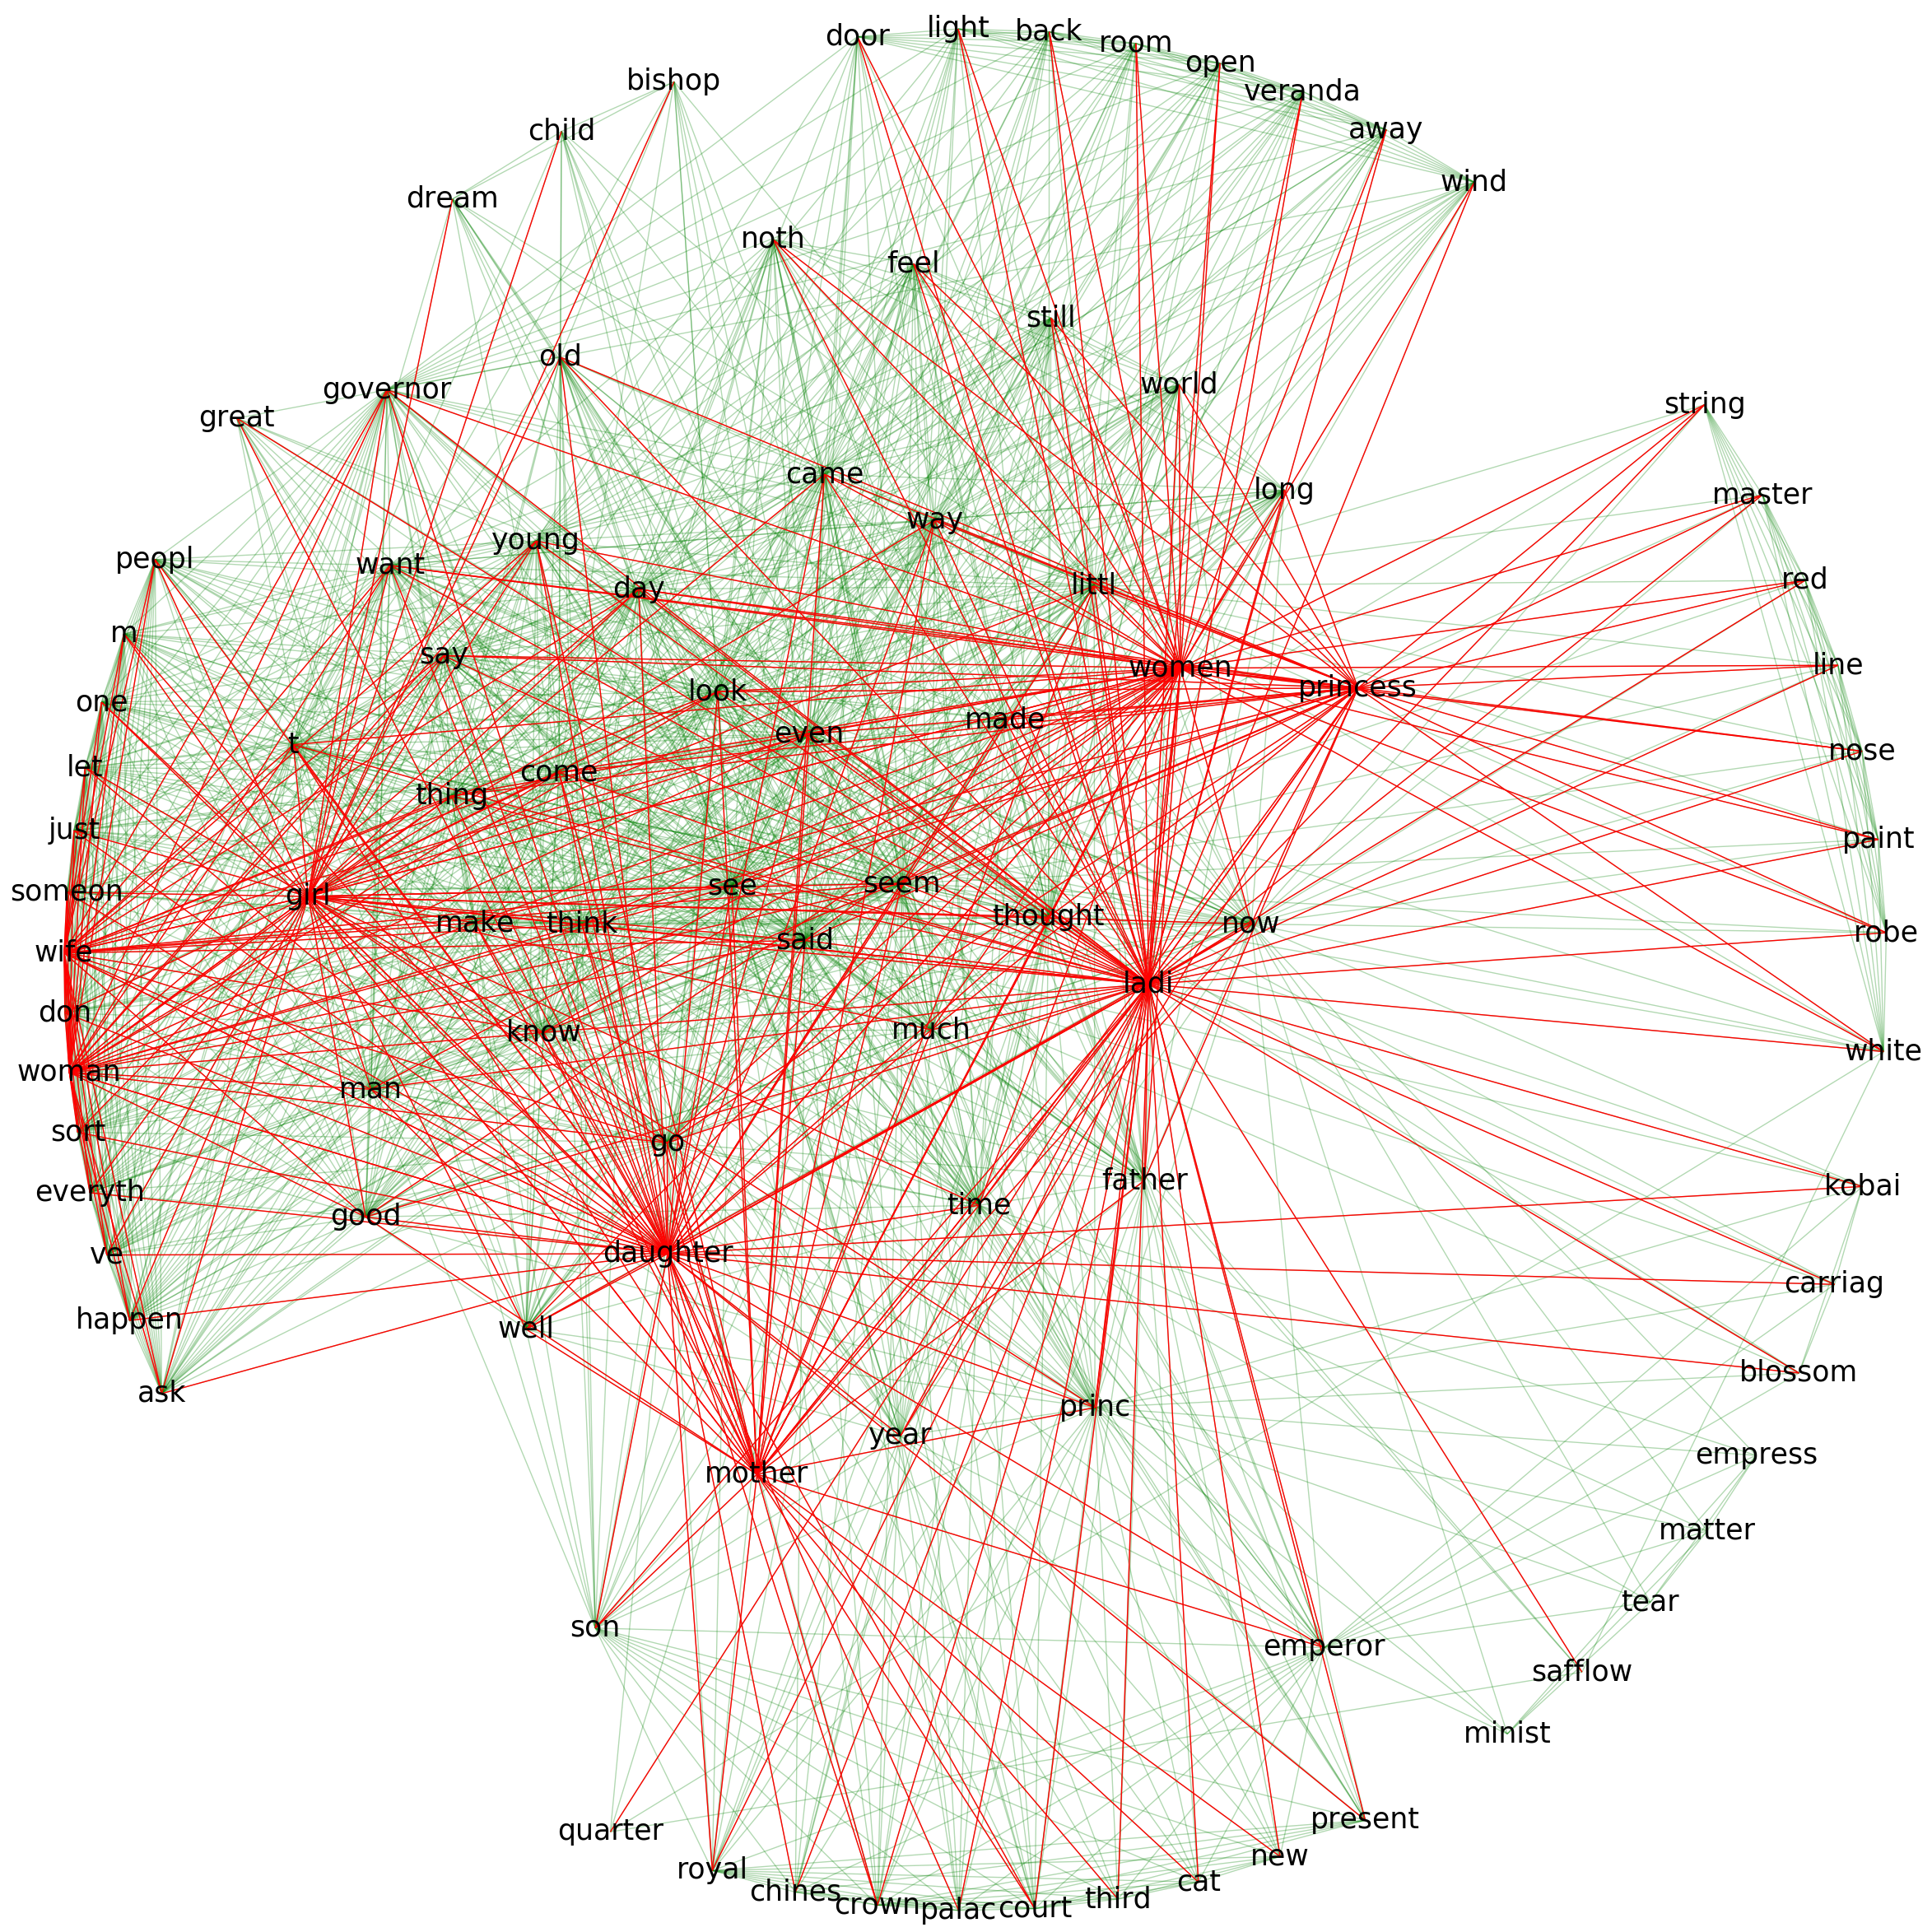
\includegraphics[width=3in]{seidensticker-complete.png}\hfill
			\caption{Seidensticker}
	  	\end{subfigure}
	\end{subfigure}\par\medskip
	\begin{subfigure}{\linewidth}
		\begin{subfigure}{.5\linewidth}
	  		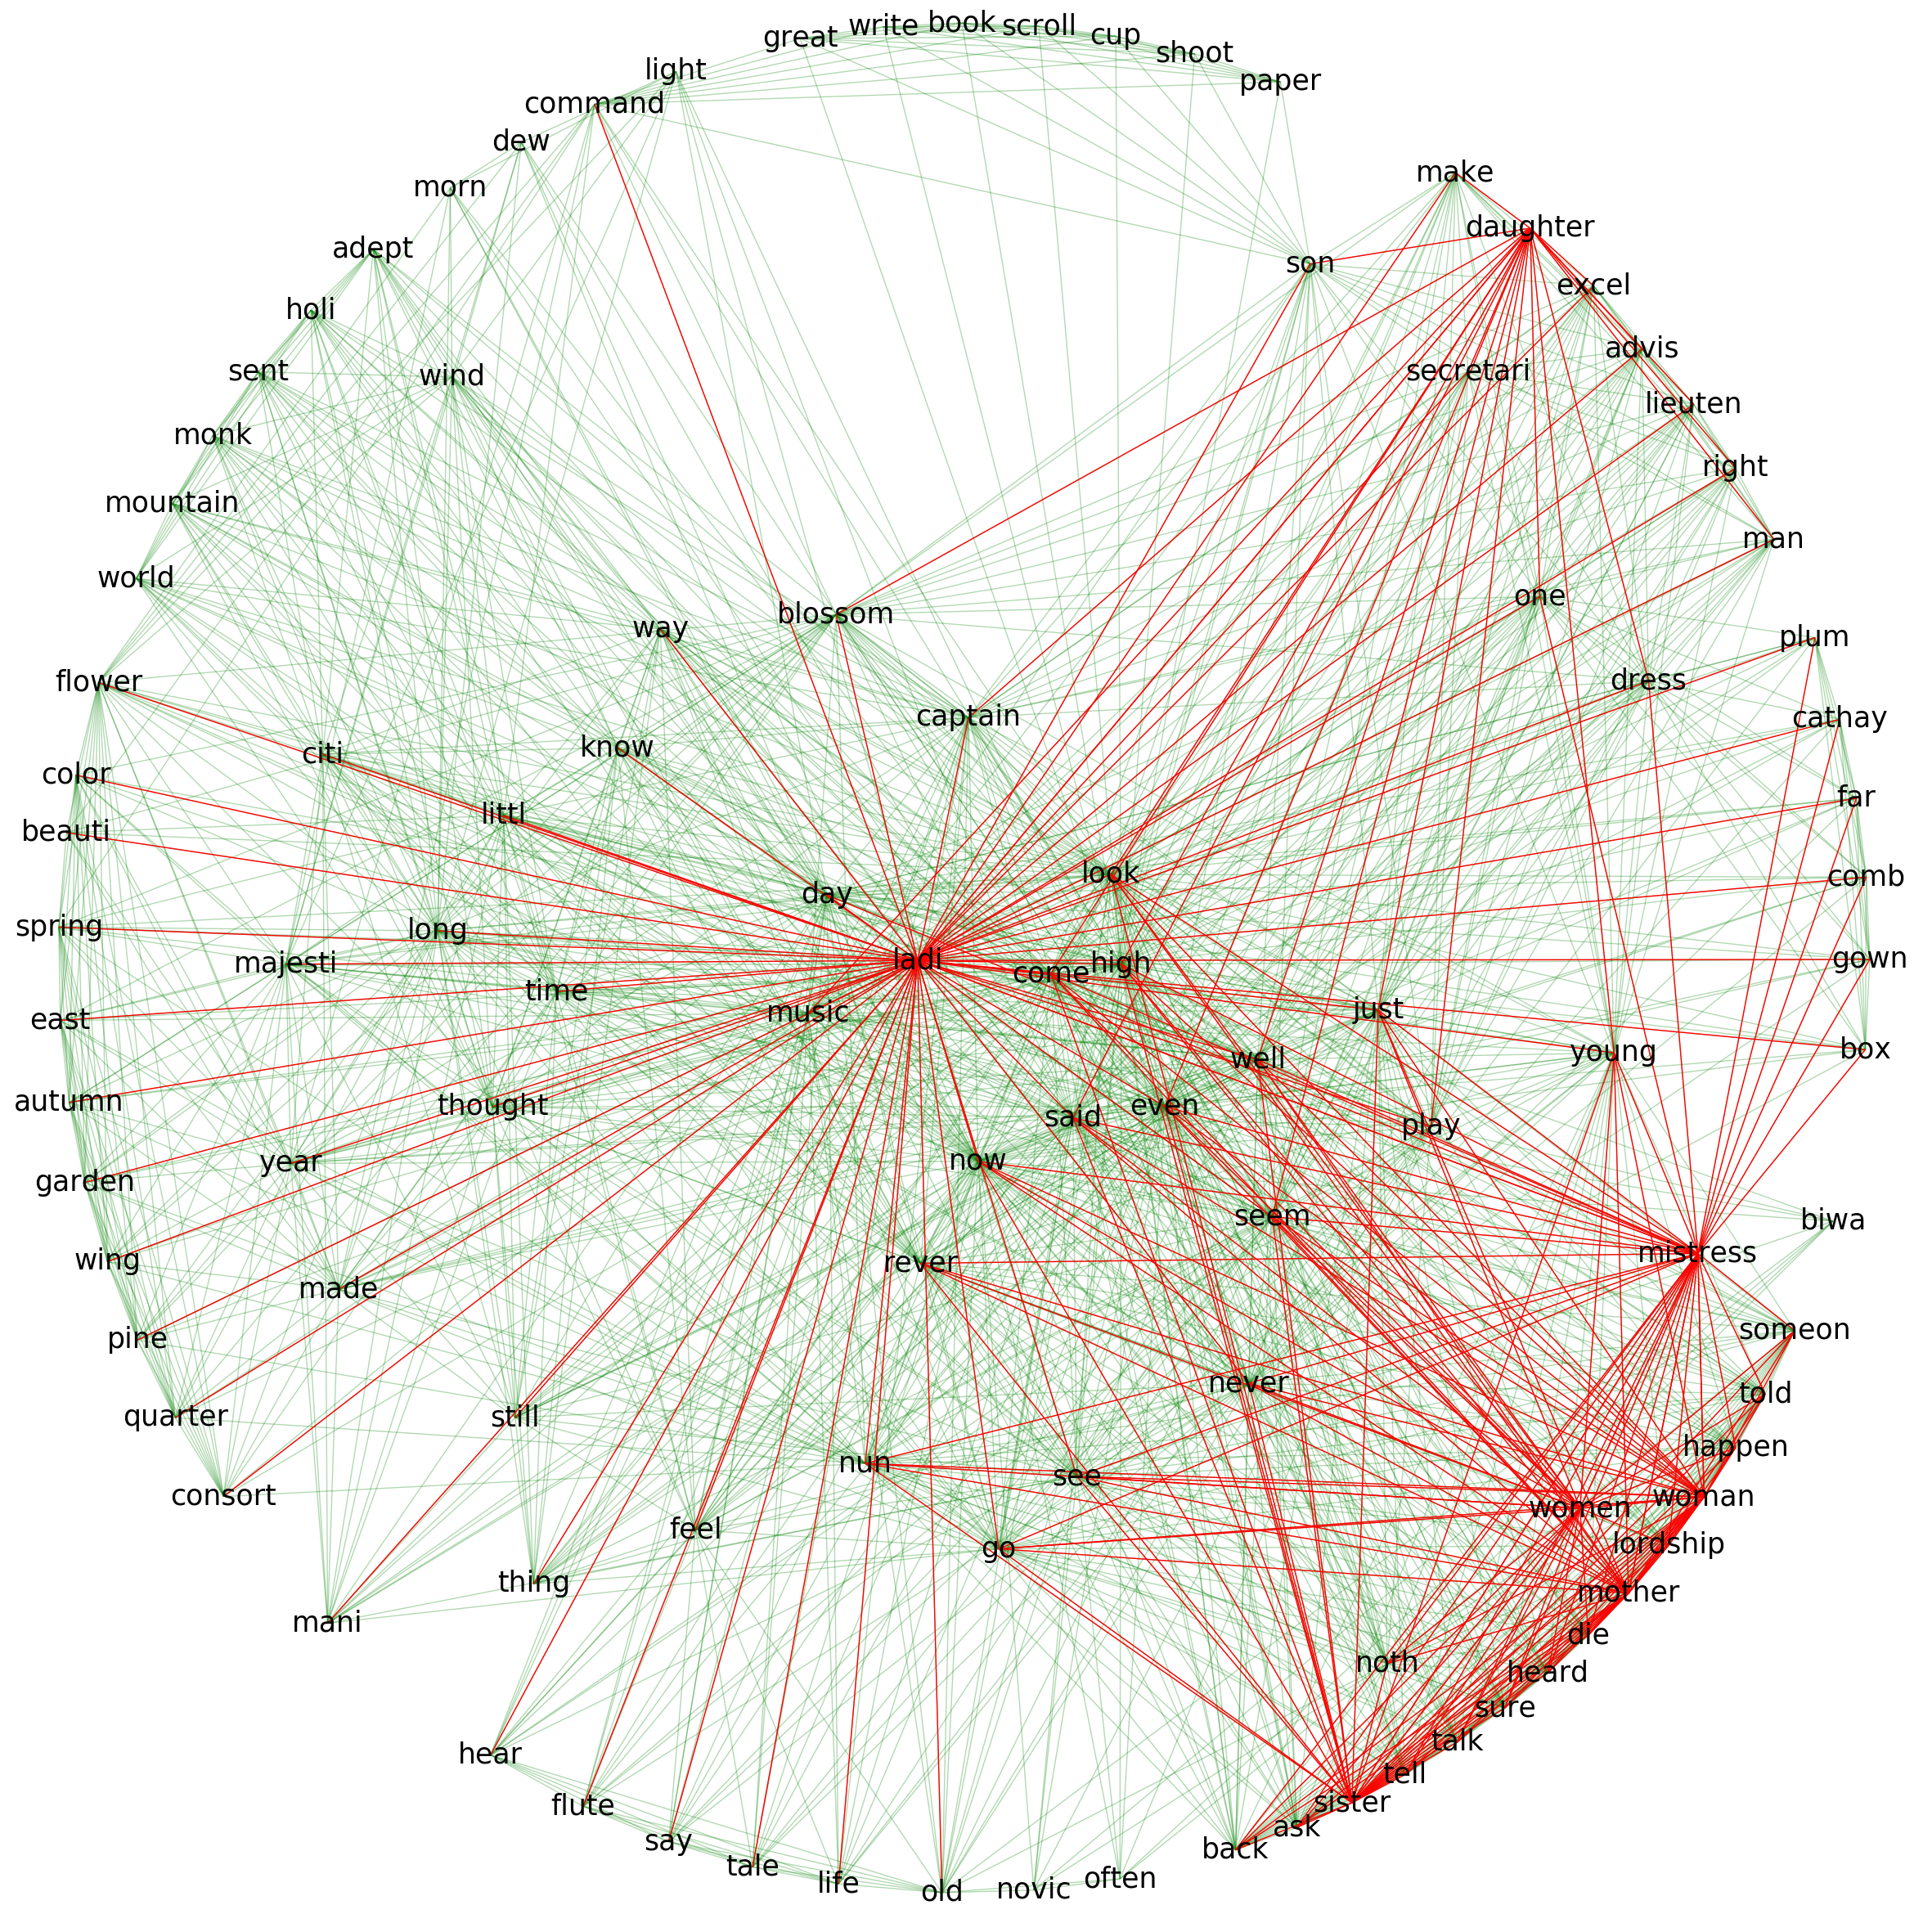
\includegraphics[width=3in]{tyler-complete.png}
	  		\caption{Tyler}
		\end{subfigure}
		\begin{subfigure}{.5\linewidth}
	  		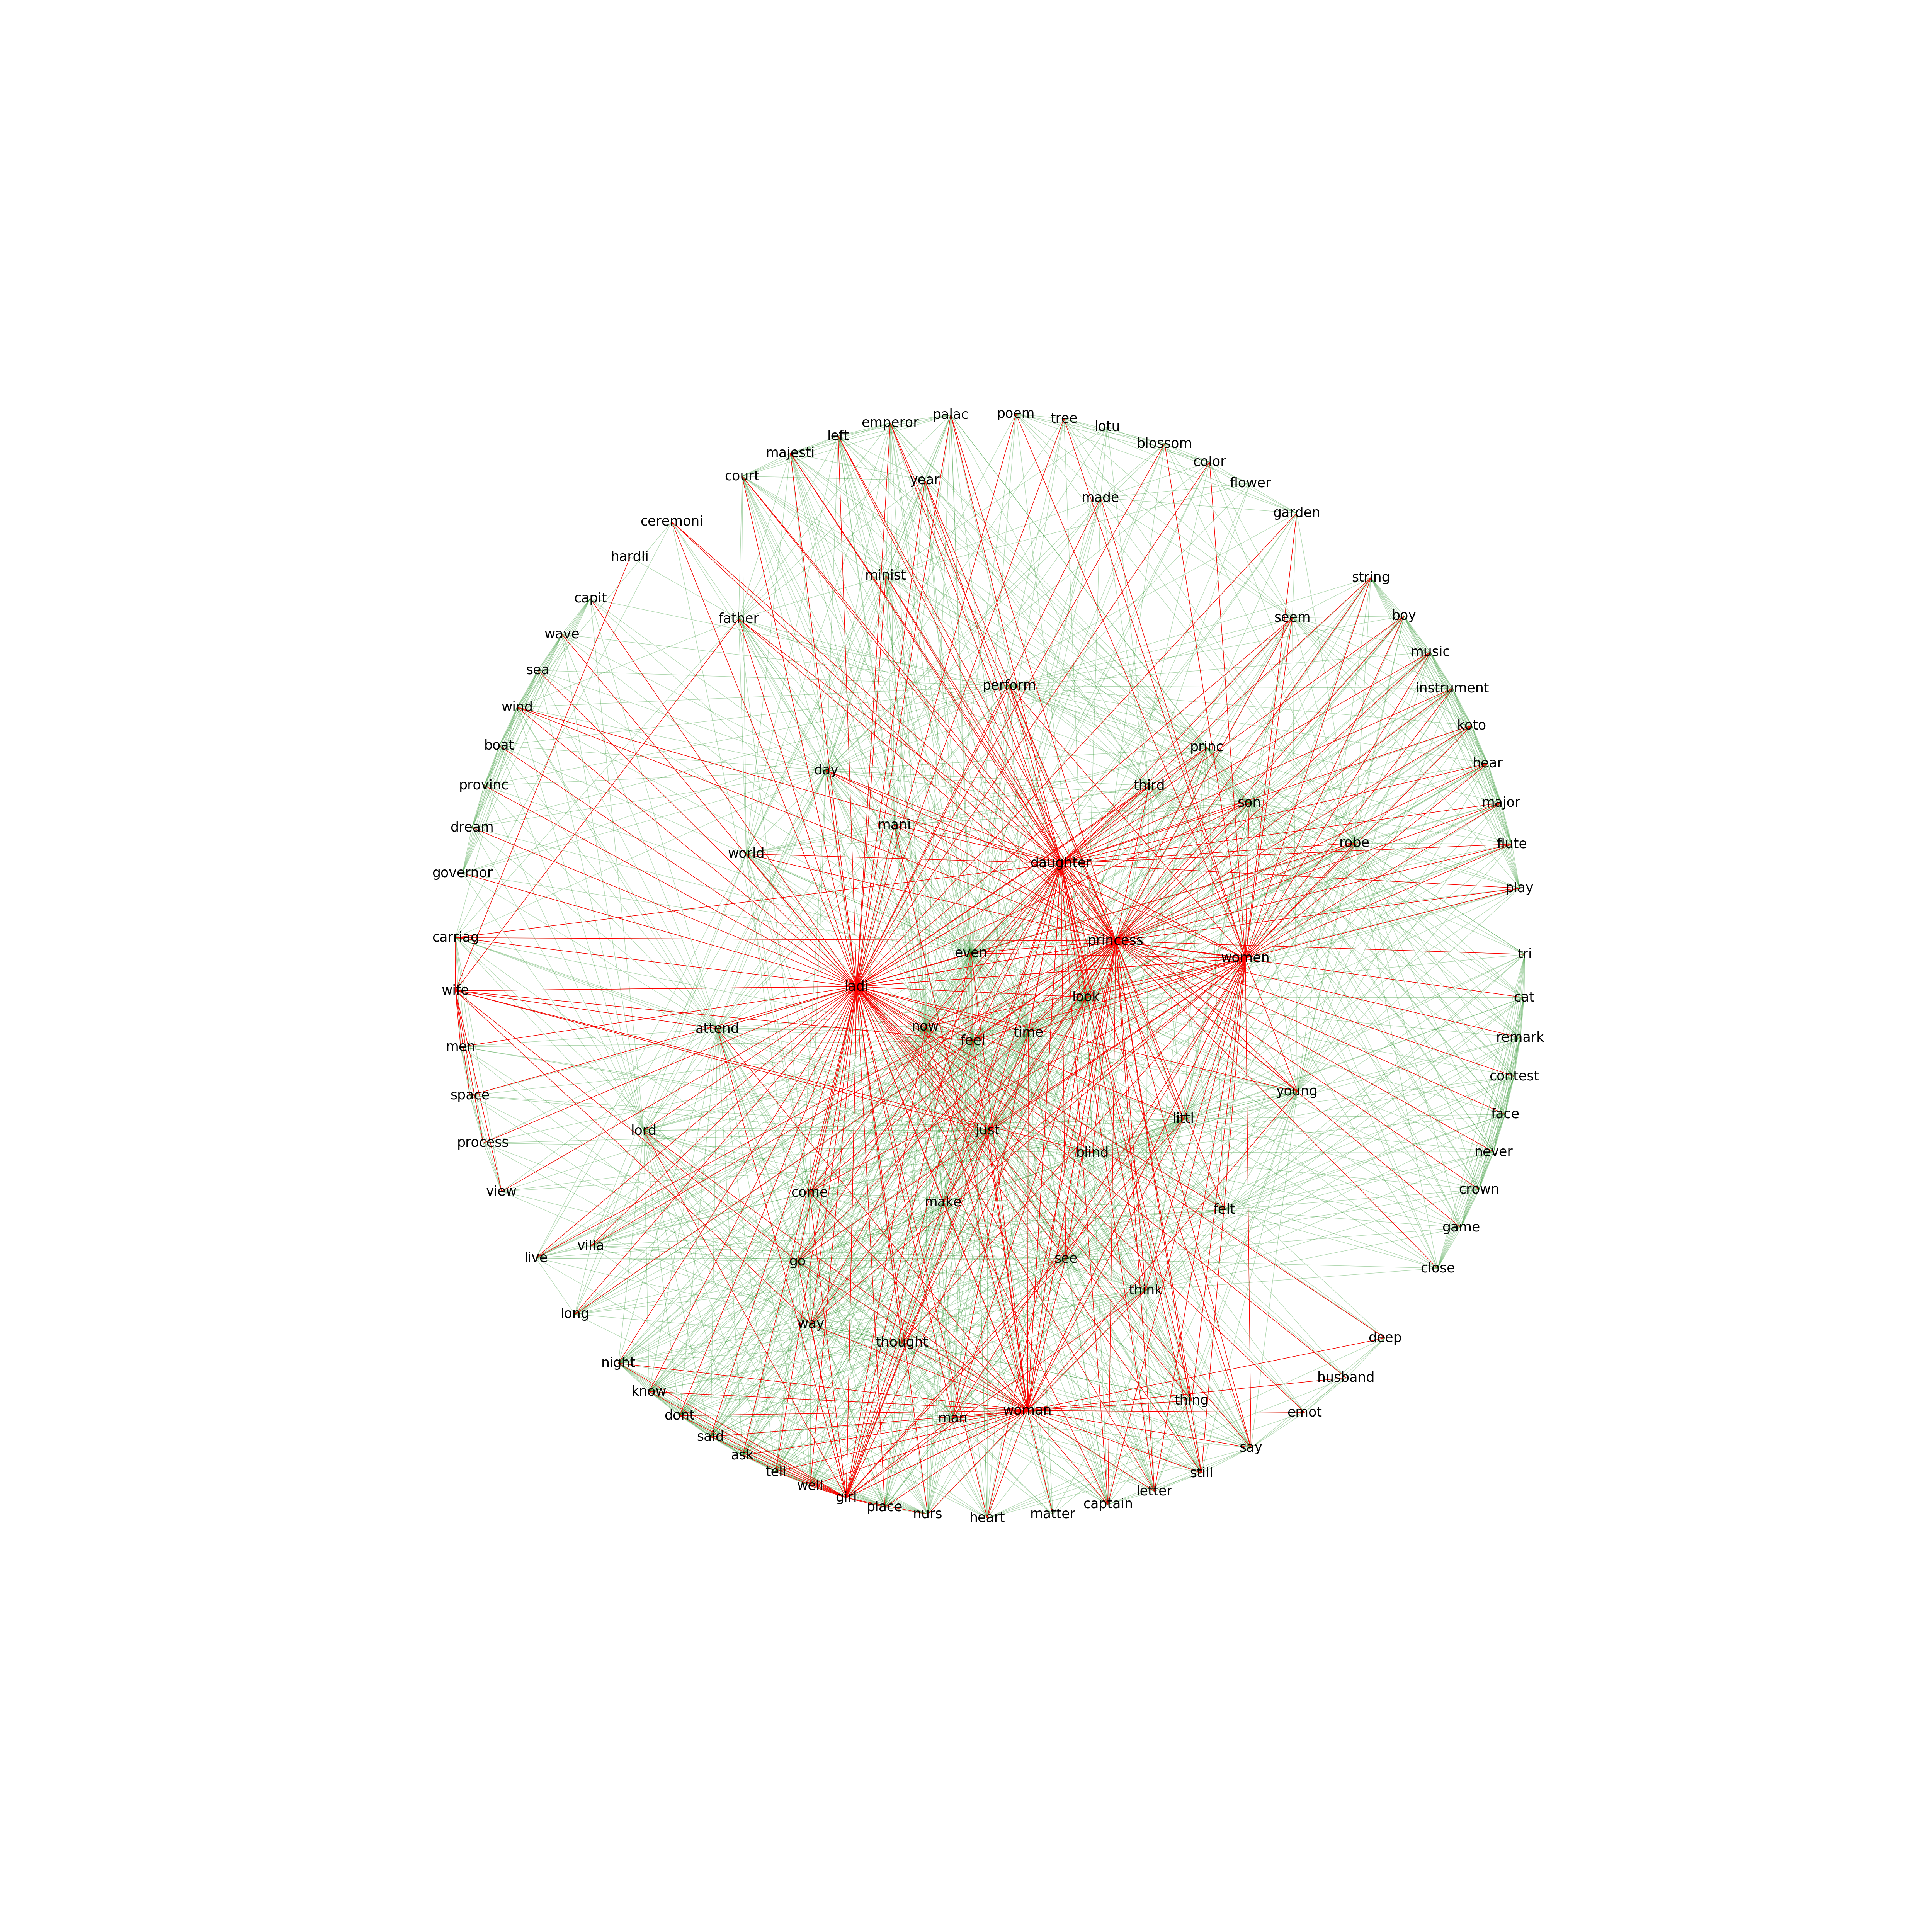
\includegraphics[width=3in]{washburn-complete.png}\hfill
	  		\caption{Washburn}
		\end{subfigure}
	\end{subfigure}
	\caption{\textit{Genji's} Thematic Structure: Female-Associated Connections in Red, Male-Associated Connections in Blue}
	\label{full-networks}
\end{figure}

The numerical observations made earlier jump out immediately now: the prevalence of women-associated words across the networks and the higher ratio of red to blue. As Moretti put it, 

\begin{displayquote}
\singlespacing
\small
``Once you make a network of a play, you stop working on the play proper, and work on a \textit{model} instead... this process of reduction and abstraction makes the model obviously much less than the original object... but also, in another sense, much \textit{more} than it,  because a model allows you to see the underlying structures of a complex object. It's like an X-ray'' (Moretti 218). 
\end{displayquote}

Beyond what is apparent via color: looking at the centrality of female and male nodes in the graph reveals that Seidensticker's and Washburn's representations of women are far more central to the thematic networks of their translations, with the female nodes having very high degrees (number of edges originating from them) and extending more uniformly across the graph. Tyler's and Waley's, on the other hand, while prevalent, are far more peripheral, suggesting a portrayal of women that is persistent yet a near afterthought, or secondary to the less frequent yet more central male occurrences. 

To probe into the dependencies and relationships that characterize this network, I follow Moretti's lead in attempting to ``\textit{intervene} on a model; make experiments (Moretti 220).'' The first is a simple one for purposes of demonstration: what happens when all women-associated nodes and the nodes that they connect to, are removed from each network, versus when all male-associated nodes are? The results are in figures \ref{networks-without-women} and \ref{networks-without-men}. The effects is apparent: in each case, the network collapses, unsurprisingly, but perhaps what is more surprising is that the removal of one word group obliterates the other as well -- both blue and red in either experiment -- showing how pervasive the distributional linkage of men and women in \booktitle{Genji} is, across translational guidelines. 

\begin{figure}
	\begin{subfigure}{\linewidth}
		\begin{subfigure}{.5\linewidth}
			\includegraphics[width=3in]{waley-no-womenwords.png}
			\caption{Waley}		
	  	\end{subfigure}
	  	\begin{subfigure}{.5\linewidth}
			\includegraphics[width=3in]{seidensticker-no-womenwords.png}\hfill
			\caption{Seidensticker}
	  	\end{subfigure}
	\end{subfigure}\par\medskip
	\begin{subfigure}{\linewidth}	  	
		\begin{subfigure}{.5\linewidth}
	  		\includegraphics[width=3in]{tyler-no-womenwords.png}\hfill
	  		\caption{Tyler}		
		\end{subfigure}
		\begin{subfigure}{.5\linewidth}
	  		\includegraphics[width=3in]{washburn-no-womenwords.png}\hfill
	  		\caption{Washburn}		
		\end{subfigure}
	\end{subfigure}
	\caption{\textit{Genji} Without Women}
	\label{networks-without-women}
\end{figure}

\begin{figure}
	\begin{subfigure}{\linewidth}
		\begin{subfigure}{.5\linewidth}
			\includegraphics[width=3in]{waley-no-menwords.png}
			\caption{Waley}		
	  	\end{subfigure}
	  	\begin{subfigure}{.5\linewidth}
			\includegraphics[width=3in]{seidensticker-no-menwords.png}\hfill
			\caption{Seidensticker}
	  	\end{subfigure}
	\end{subfigure}\par\medskip
	\begin{subfigure}{\linewidth}	  	
		\begin{subfigure}{.5\linewidth}
	  		\includegraphics[width=3in]{tyler-no-menwords.png}\hfill
	  		\caption{Tyler}		
		\end{subfigure}
		\begin{subfigure}{.5\linewidth}
	  		\includegraphics[width=3in]{washburn-no-menwords.png}\hfill
	  		\caption{Washburn}		
		\end{subfigure}
	\end{subfigure}
	\caption{\textit{Genji} Without Men}
	\label{networks-without-men}
\end{figure}

Examining the non-gendered (as we may currently believe) nodes central to the graphs reveals fruitful direction for future experiments. 'feel' is the most central node in the Washburn graph, with 'thought' being a close second. 'Perform', 'attend', and 'robe' introduce the element of appearance and service. In Tyler, ceremonial words like 'rever', 'music', 'play', 'majesti' and 'high' occur with high degrees, Waley's has similar trends with 'palace' and 'prince', and Seidensticker's features 'look', 'governor', and 'long'. From these observations, we can identify three major categories as bases for interrogating the model. Feeling and thinking: 'feel', 'think', 'felt', 'thought', 'tear', 'emot', 'die', performance and appearance: 'perform', 'play', 'dress', 'robe', 'music', and duty and court: 'palace', 'ceremoni', 'attend', 'rever', 'crown'.



The most intriguing changes, however, are when we remove individual female words rather than all female words in their entirety. Removal of the word 'mother' has different effects on each network, reducing Seidensticker's to a notably more romantic, sentimental, and courtship-heavy structure. In Waley's case, removal of the word "mother" results in

Removing feeling and thinking words, specifically 'feel', 'felt', 'think', 'thought', 'emot', removes all mention of females from Seidensticker's network.

Removing duty and palace-related words reduces the female network of Tyler almost exclusively to independent women-words, and removal of feeling-thinking words reduces the network almost entirely to male-independent women.


In the Washburn text, the word ``feel'' is the second-most salient one in the entire novel. The topic-modeling results reveal that the word ``feel'' occurs exclusively in the female-related themes, and is mentioned not once in a female-unrelated theme. Additionally, while five of the female-related themes also mention male-related words in them, only one of these contains the word ``feel.'' [This demonstrates that the inner life of women is given priority in Washburn's translation, and more importantly, in contexts where women are not surrounded by other men. Females are afforded a level of individuality that they are not in the other translations.] TODO comment was''This is where ``microanalysis'' (using human brain power) can come back in to make a contribution in supporting the contours of the big data [see end comments]''. This is evident in the Tyler translation, where the word majestic appears in four out of eight of the female themes (specifically the ones on courtship and ceremony), and only three times in all the other twelve, thereby indicating the presence of females as a cultural object for the purposes of courtly procedure and order. The Waley translation, by far, exhibits the most striking objectification and minimization of women --- women occur explicitly in themes about ceremony, palaces, and governance, thereby indicating a position in the text that is secondary to their male fathers and husbands. [TODO COMMENT: Similarly insightful. To extend the point for maximum impact: what do these additional associations tell us about the nature of that ``objectification and minimization''? i.e., the switch from an adjective or quality of class (``majestic'') to a set of physical places and cultural practices (``ceremony''). Ceremony appears in both Tyler and Waley, so how might it function differently in each?]

\begin{workscited}

\bibent Jockers, M. L..\booktitle{Macroanalysis: Digital Methods and Literary History}. Champaign: University of Illinois Press, 2013. Project MUSE.

\bibent Rhody, Lisa M. ``Topic Modeling and Figurative Language.'' \booktitle{Journal of Digital Humanities}, vol. 2, no. 1, 2012, pp. 19---38.

\bibent Henitiuk, Valerie. ``Going to Bed with Waley: How Murasaki Shikibu does and does not become world literature.'' \booktitle{Comparative Literature Studies}, vol. 45, no. 1, 2008, pp. 40---61., www.jstor.org/stable/25659632.

\bibent Shikibu, Murasaki, and Dennis C. Washburn. \booktitle{The Tale of Genji}. New York: W.W. Norton, 2015. Amazon.com. Web.

\bibent Shikibu, Murasaki, and Arthur Waley. \booktitle{The Tale of Genji}. Boston and New York: Houghton Mifflin, 1925. Amazon.com. Web.

\bibent Murasaki Shikibu B. ''University of Oxford Text Archive.'' [OTA] \booktitle{The Tale of Genji} [Electronic Resource]. Trans. Edward G. Seidensticker. N.p., n.d. Web. 16 Apr. 2017. http://ota.ox.ac.uk/desc/2245.

\bibent Murakami, Janel R. Goodman. ''Metonymy in The Tale of Genji: An Analysis of Translation Strategies.'' \booktitle{Arizona Working Papers in SLA and Teaching 20} (2013): 55-75.

\bibent Moretti, Franco. ``Network Theory, Plot Analysis.'' \booktitle{Distant Reading}. London: Verso, 2015. N. pag. Print.

\bibent Childs, M. H. (1999). The value of vulnerability: Sexual coercion and the nature of love in japanese court literature. \booktitle{The Journal of Asian Studies}, 58(4), 1059-1079. Retrieved from http://search.proquest.com.ezp-prod1.hul.harvard.edu/docview/230413728?accountid=11311
\end{workscited}


\end{spacing}
\end{flushleft}
\end{document}
